\subsection{Past experiments on similar PSCs}
The combination of 2D and 3D perovskite structures has been an area of interest for researchers for some time. In addition, multiple organics have been used to create new and improved materials. These types of combinations have been previously documented and are summarized in Table 2.1.
\begin{table}[htb]
\caption{Summary of past experiments on similar PSCs.}
\begin{adjustbox}{max width=1\textwidth,center}
\begin{tabular}{c c c c}
\hline
    \textbf{Perovskite material} & \textbf{Architecture} & \textbf{PCE (\%)} & \textbf{Ref}\\ \hline
    (PEA)\textsubscript{2}(MA)\textsubscript{2}Pb\textsubscript{3}I\textsubscript{10}           & FTO/c-TiO\textsubscript{2}/perovskite/spiro-OMeTAD/Au  & 4.73  & {\cite{smith_layered_2014}} \\ \hline
    (BA)\textsubscript{2}(MA)\textsubscript{2}Pb\textsubscript{2}I\textsubscript{2}            & FTO/mp-TiO\textsubscript{2}/perovskite/spiro-OMeTAD/Au & 4.02  & {\cite{cao_2d_2015}} \\ \hline
    (BA)\textsubscript{2}(MA)\textsubscript{3}Pb\textsubscript{4}I\textsubscript{13}            & FTO/mp-TiO\textsubscript{2}/perovskite/spiro-OMeTAD/Au & 2.39  & {\cite{cao_2d_2015}} \\ \hline
    (IC\textsubscript{2}H\textsubscript{4}NH\textsubscript{3})\textsubscript{2}(MA)\textsubscript{n–1}Pb\textsubscript{n}I\textsubscript{3n+1}  & FTO/mp-TiO\textsubscript{2}/perovskite/spiro-OMeTAD/Au & 9.03  & {\cite{koh_nanostructuring_2016}}\\ \hline
    (AVA)\textsubscript{x}(MA)\textsubscript{1−x}PbI\textsubscript{3}           & FTO/mp-TiO\textsubscript{2}/mp-ZrO\textsubscript{2}/perovskite/carbon  & 11.86 & {\cite{saparov_organicinorganic_2016}}\\ \hline
    (PEA)\textsubscript{2}(MA)\textsubscript{49}Pb\textsubscript{50}Br\textsubscript{151}       & FTO/mp-TiO\textsubscript{2}/perovskite/spiro-OMeTAD/Au & 8.5   & {\cite{cohen_high_2017-1}} \\ \hline
    (PPA)\textsubscript{2}(MA)\textsubscript{49}Pb\textsubscript{50}Br\textsubscript{151}       & FTO/mp-TiO\textsubscript{2}/perovskite/spiro-OMeTAD/Au & 7.1   & {\cite{cohen_high_2017}} \\ \hline
    (BZA)\textsubscript{2}(MA)\textsubscript{49}Pb\textsubscript{50}Br\textsubscript{151}       & FTO/mp-TiO\textsubscript{2}/perovskite/spiro-OMeTAD/Au & 9.5   & {\cite{cohen_high_2017} \\ \hline
    (EDA)(MA)\textsubscript{2}{[Pb\textsubscript{3}I\textsubscript{10}]}      & FTO/mp-TiO\textsubscript{2}/perovskite/spiro-OMeTAD/Au & 11.58 & {\cite{jiang_new_2016} \\ \hline
    GAMA\textsubscript{3}Pb\textsubscript{3}I\textsubscript{10}                 & FTO/PEDOT:PSS/perovskite/PCBM/Al       & 7.26  & {\cite{soe_new_2017}} \\ \hline
    (PEI)\textsubscript{2}(MA)\textsubscript{6}Pb\textsubscript{7}I\textsubscript{22}           & ITO/PEDOT:PSS/perovskite/PCBM/LiF/Ag   & 9.39  & {\cite{yao_multilayered_2016}} \\ \hline
    (BA)\textsubscript{2}(MA)\textsubscript{3}Pb\textsubscript{4}I\textsubscript{13}   (HC)     & FTO/PEDOT:PSS/perovskite/PCBM/Al       & 12.51 & {\cite{tsai_high-efficiency_2016}} \\ \hline
    (iso-BA)\textsubscript{2}(MA)\textsubscript{3}Pb\textsubscript{4}I\textsubscript{13}   (HC) & ITO/C\textsubscript{60}/perovskite/spiro-OMeTAD/Au     & 10.63 & {\cite{chen_tailoring_2017}} \\ \hline
    (BA)\textsubscript{2}(MA)\textsubscript{3}Sn\textsubscript{4}I\textsubscript{13}            & FTO/m-TiO\textsubscript{2}/perovskite/PTAA:TPFB/Au      & 2.53  & {\cite{cao_thin_2017}} \\ \hline
    PEA\textsubscript{2}FA\textsubscript{8}Sn\textsubscript{9}I\textsubscript{28}               & ITO/NiO\textsubscript{x}/perovskite/PCBM/Al            & 5.94  & {\cite{liao_highly_2017}} \\ \hline
    (PEA)\textsubscript{2}(FA)\textsubscript{n−1}Sn\textsubscript{n}I\textsubscript{3n+1}       & ITO/PEDOT:PSS/perovskite/C\textsubscript{60}/BCP/Al    & 9.0   & {\cite{shao_highly_2018}} \\ \hline
\end{tabular}
\end{adjustbox}
\end{table}
\par \subsection{Device structure}
PSCs are configured in such a way as to maximize power conversion. Solar cells worked on the principle of the photoelectric effect, making the light-harvesting layer the core component of solar cells. Absorption of light occurs within the light-harvesting layer, where an electron when excited becomes an electron-hole pair.
The device architecture of a perovskite solar cell typically consists of several layers of materials that are arranged in a specific way to allow the cell to efficiently convert sunlight into electricity. The exact composition of these layers can vary depending on the specific type of perovskite solar cell, but typically they include the following a transparent conductive layer on the front of the cell or front contact, which allows sunlight to pass through and also acts as an electrical conductor, a layer of perovskite material, which absorbs sunlight and generates charge carriers (electrons and holes) as a result, a layer of electron-transport material (ETM), which helps to collect and transport the electrons generated by the perovskite layer, a layer of hole-transport material (HTM), which helps to collect and transport the holes generated by the perovskite layer, a layer of metal on the back of the cell or back contact, which acts as a conductor and helps to collect the charge carriers generated by the perovskite layer. The structure is illustrated in Figure 2.1.
\begin{figure}[H]
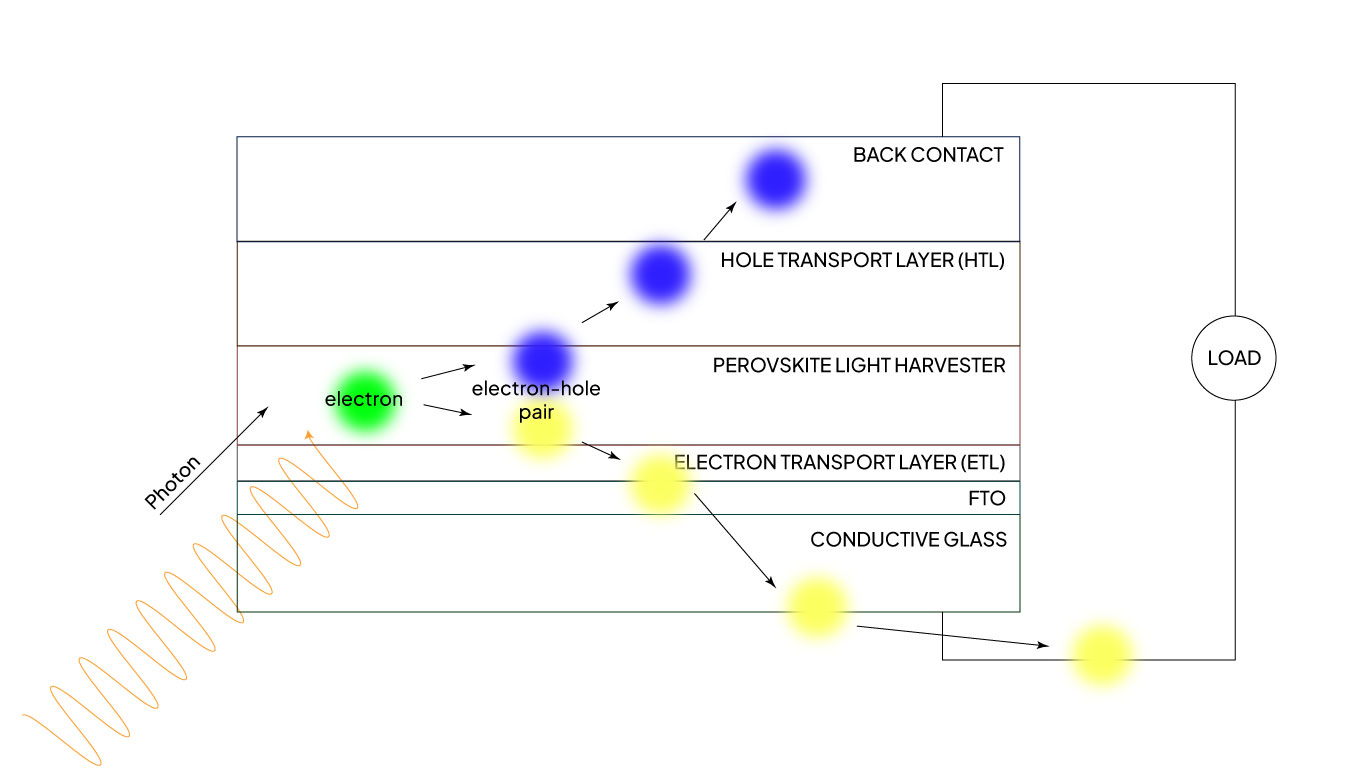
\includegraphics[width=14 cm]{img-content/psc-mechanism2.jpg}
\caption{Structure of a perovskite solar cell. Both glass (conductive) and Fluorine Tin Oxide (FTO) coat can also be collectively called as front contact. A wire connecting back and front contact can be placed to allow electron to flow\label{fig1}}
\end{figure}   
